\documentclass{article}
\usepackage[utf8]{inputenc}

\usepackage{natbib}
\usepackage{amsthm}
\usepackage{amssymb}
\usepackage{float}
\usepackage{algorithm}
\usepackage{algpseudocode}

\usepackage{amsmath}%
\usepackage{MnSymbol}%
\usepackage{wasysym}%
\usepackage{graphicx}
\usepackage{csquotes}
\usepackage{geometry}
 \geometry{
 a4paper,
 total={170mm,257mm},
 left=30mm,
 right=30mm,
 top=20mm,
 }
\newcommand{\argmax}{\arg\!\max}
\newcommand*{\QEDA}{\hfill\ensuremath{\blacksquare}}%

\begin{document}
\begin{titlepage}
\begin{center}

\vspace*{10cm}
{\large Master 1 MoSIG}\\[0.5cm]

{\Huge \textbf{Algorithmic Problem Solving} }\\[0.5cm]
{\large APP3 Report}\\
Hole Drilling\\ 
Team:\\SACAD
\vfill

% Author and supervisor
\noindent
\begin{minipage}{0.4\textwidth}
   \centering Members:\\
   Andrey \textbf{SOSNIN}\\
   Majdeddine \textbf{ALHAFEZ}\\
   Antoine \textbf{COLOMBIER}\\
   Eman \textbf{AL-SHAOUR}\\
   Son Tung \textbf{DO}\\
\end{minipage}%

\vfill
% Bottom of the page
{Grenoble, 12 November, 2017}
\end{center}
\end{titlepage}
\clearpage

\section{Discussion on the current algorithm}


\subsection{Not an $\alpha$-approximation}
Let us assume that we have $N$ points to drill and they are arranged as shown in figure1 where the distance between two horizontal points equals $2N$ and the distance between two vertical points equals to $1$.

\begin{figure}[h]
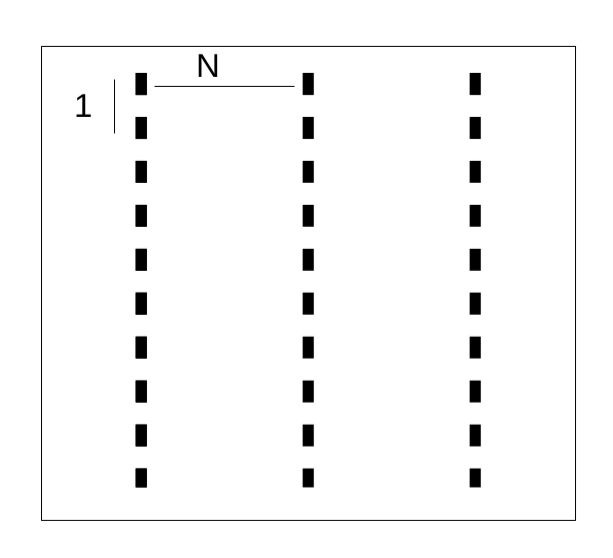
\includegraphics[width=0.3\linewidth]{F0.jpg}
\caption{circuit board}
\end{figure}

\begin{figure}[h]
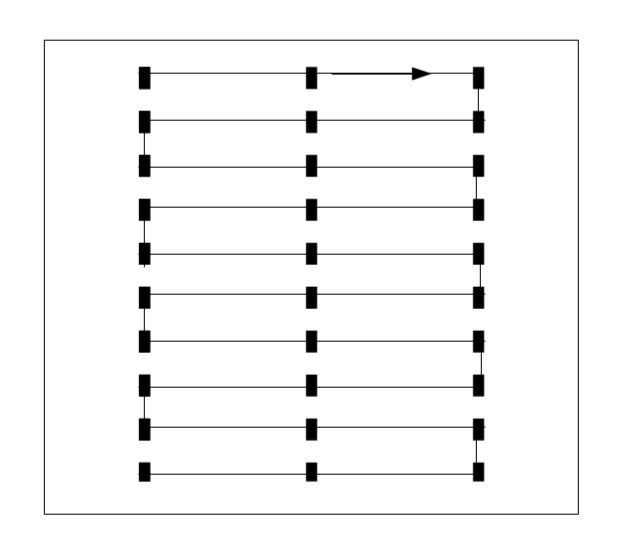
\includegraphics[width=0.3\linewidth]{F1.jpg}
\caption{behavior of the current algorithm}
\end{figure}

\begin{figure}[h]
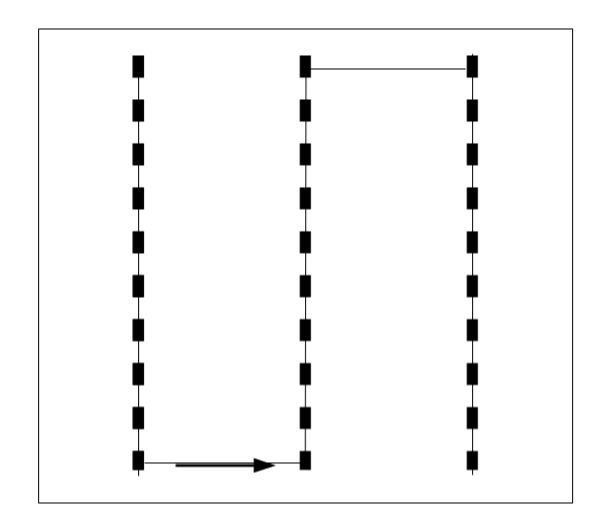
\includegraphics[width=0.3\linewidth]{F2.jpg}
\caption{behavior of the greedy algorithm}
\end{figure}

Figure 2 shows the behavior of the current algorithm (this is the best behavior where after drilling all the points in a row, we drill the point just bellow the last drilled point). The total cost of the algorithm is 
$C = $O($N^{2}$)

Figure 3 shows the behavior of what seems to be a better solution where we have $C* = $O($N$)
The ratio is $C = $O($N$) and therefore such $\alpha$ doesn't exist and the current algorithm is not an $\alpha$-approximation.

\section{Greedy Approach}
\subsection{Propose an algorithm}
This greedy approach consists of going through the set of points picking up the point with the minimum distance to the current point.

\begin{algorithm}[H]
\caption{Greedy}
\textbf{Input: }$A[N]$ array of N points to drill\\
\textbf{Output: }the order in which we drill the points
\begin{algorithmic} 
\For{\texttt{k from 0 to N}}
    \State $index \leftarrow -1$
    \State $min\_distance \leftarrow \infty $
    \For{\texttt{i from k+1 to N}}
        \State $distance \leftarrow find\_distance(A[k], A[i])$
        \If{$ distance < min\_distance$}
            \State $index = i$ 
            \State $min\_distance \leftarrow distance$
        \EndIf
    \EndFor
    \State $swap\_elements(k+1, index)$
\EndFor

\end{algorithmic}
\end{algorithm}
The function $find\_distance(p1, p2)$ calculate the Euclidean distance between two points which is given by:
$distance = \sqrt{(x1-x2){^2} + (y1+y2)}{^2} $

\subsection{Showing it is not optimal}
\subsection{Proof it is a 2-approximation}
\subsection{Proof it is not a 2-approximation}

\section{Minimum Spanning Tree}

\subsection{Propose an algorithm}

\subsection{2-approximation proof}
We know that every spanning tree is more expensive than the weight of the MST, thus making a lower bound regarding the optimal solution :\\
$MST \leq C{^*}$ \\
Our algorithm consider the MST of the the holes, in the worst case, we go through every edge in MST twice\\
$C = 2 * MST$ \\ 
We conclude that the algorithm is a 2-approximation.

\section{Kruskal's/Prim's Algorithm}

\end{document}

